\section{Breve historia de la formulación de la mecánica cuántica}

    El capítulo anterior terminó con la ecuación de Schrödinger y con la integral de camino, es decir, con dos maneras distintas de escribir la dinámica cuántica, pero sin haber dicho en ningún momento qué es lo que evoluciona ni qué relación guarda con lo que se mide en un laboratorio. Esa omisión no es un descuido de la exposición sino un reflejo fiel de la historia: la mecánica cuántica se construyó primero como un conjunto de reglas de cálculo que funcionaban, y solo después, y con considerable esfuerzo, se le encontró una estructura matemática coherente y una interpretación. Este capítulo recorre esa estructura y esa interpretación, porque sin ellas el capítulo siguiente, en el cual promoveremos las amplitudes del campo electromagnético a operadores, sería una manipulación formal sin contenido.

    El punto de partida es el verano de 1925 y un joven de veintitrés años enfermo de fiebre del heno. Werner Heisenberg, refugiado en la isla de Helgoland para escapar del polen, decidió abandonar por completo el intento de describir la órbita del electrón y construir una teoría que se refiriese únicamente a cantidades observables, es decir, a las frecuencias y a las intensidades de las líneas espectrales \citep{heisenberg1925umdeutung}. El resultado fue un esquema de cálculo en el que a cada observable le corresponde una tabla doblemente indexada de números, y en el que el producto de dos tablas no conmuta. Heisenberg no sabía que estaba multiplicando matrices; fue Max Born quien lo reconoció al leer el manuscrito, y quien junto con Pascual Jordan escribió la teoría en forma matricial y descubrió la relación fundamental \citep{bornjordan1925zur}
    \begin{equation}\label{eq:ConmutadorHistorico}
        \hat{q}\hat{p} - \hat{p}\hat{q} = i\hbar\,\mathbb{1},
    \end{equation}
    que apareció así, en noviembre de 1925, antes de que existiera ninguna función de onda y sin ninguna interpretación clara de qué era lo que representaba. La versión definitiva del formalismo matricial, extendida a sistemas de varios grados de libertad, se publicó pocos meses después en el célebre trabajo de los tres autores \citep{bornheisenbergjordan1926}.

    En enero de 1926 Schrödinger publicó, como vimos, una teoría completamente distinta en apariencia, basada en una ecuación diferencial para una función de onda continua \citep{schrodinger1926quantisierung}. La coexistencia de dos formalismos que producían los mismos números pero que no se parecían en nada resultaba intolerable, y el propio Schrödinger demostró ese mismo año la equivalencia entre ambos \citep{schrodinger1926verhaltnis}, mostrando que las matrices de Heisenberg son los elementos de matriz de operadores diferenciales entre las funciones propias de su ecuación. La demostración era correcta en el espíritu aunque incompleta en el rigor, y la versión definitiva de la equivalencia, junto con la estructura que hoy llamamos teoría de transformaciones, es obra de Dirac en 1927 \citep{dirac1927physical}.

    Faltaba, sin embargo, lo esencial. Schrödinger creía que $|\psi|^{2}$ describía una densidad de carga real, una especie de nube material extendida, y defendió esa lectura durante años pese a la objeción evidente de que el paquete de ondas de una partícula libre se ensancha indefinidamente mientras que un electrón nunca se observa dividido. La interpretación correcta la propuso Born en junio de 1926, en un artículo sobre colisiones atómicas, y lo hizo en una nota a pie de página añadida durante la corrección de pruebas: $|\psi|^{2}$ no es una densidad de materia sino una \textit{densidad de probabilidad} \citep{born1926stossvorgange}. \textbf{Aquella nota al pie, que Born escribió casi como una enmienda de último momento, es probablemente la frase más consecuente de toda la física del siglo XX}, porque introdujo el azar en el nivel fundamental de la descripción y cambió para siempre el estatus de las leyes físicas. Born recibió el premio Nobel por ella en 1954, veintiocho años después.

    El año siguiente trajo los dos resultados que fijaron el significado físico del formalismo. Heisenberg publicó en 1927 su análisis de lo que puede saberse simultáneamente sobre la posición y el momento de una partícula \citep{heisenberg1927anschaulichen}, obteniendo la relación de indeterminación mediante un argumento sobre el microscopio de rayos gamma que, como veremos, es sugerente pero engañoso; Earle Kennard demostró ese mismo año la versión rigurosa para el caso canónico \citep{kennard1927quantenmechanik} y Howard Robertson la generalizó en 1929 a cualquier par de observables \citep{robertson1929uncertainty}. Y Niels Bohr presentó en el congreso de Como su principio de complementariedad \citep{bohr1928quantum}, según el cual las descripciones ondulatoria y corpuscular no se contradicen sino que se excluyen mutuamente en cada montaje experimental concreto, tesis que sigue siendo el núcleo de la llamada interpretación de Copenhague.

    La arquitectura matemática definitiva llegó en 1932 de la mano de John von Neumann, quien en \textit{Mathematische Grundlagen der Quantenmechanik} demostró que el espacio de funciones de onda de Schrödinger y el espacio de sucesiones de Heisenberg son dos realizaciones del mismo objeto abstracto, un espacio de Hilbert separable, y reformuló toda la teoría en ese lenguaje \citep{vonneumann1932mathematische}. Von Neumann introdujo también, en un trabajo previo de 1927 \citep{vonneumann1927wahrscheinlichkeitstheoretischer} y de manera independiente a Landau, quien llegó al mismo objeto estudiando la emisión espontánea \citep{landau1927dampfungsproblem}, la matriz densidad, que es la herramienta imprescindible cuando el sistema no se encuentra en un estado puro. Esa herramienta, que en su origen era un tecnicismo para tratar subsistemas y mezclas estadísticas, resultó ser el objeto central de la óptica cuántica, porque la luz que emiten las fuentes reales, desde una bombilla hasta una estrella, nunca está en un estado puro.

    El orden de exposición que seguiremos invierte el orden histórico, como es habitual y conveniente. Enunciaremos primero la estructura del espacio de estados, después los postulados en su forma moderna, junto con su interpretación física y con las objeciones que cada uno suscita, y a continuación los resultados que necesitaremos más adelante: el principio de indeterminación, las representaciones de posición y momento, las imágenes de evolución, el oscilador armónico resuelto algebraicamente y, para terminar, la matriz densidad y su conexión con la teoría de la coherencia del capítulo segundo.

\section{El espacio de estados}

        Toda la mecánica cuántica se desarrolla sobre una estructura matemática única, y la definimos con precisión antes de colgar de ella ninguna física.

        \begin{myDef}\label{def:Hilbert}
            Un \textit{espacio de Hilbert} $\mathcal{H}$ es un espacio vectorial sobre el cuerpo de los números complejos, dotado de un producto interno $\langle\cdot\,|\,\cdot\rangle : \mathcal{H}\times\mathcal{H}\rightarrow\mathbb{C}$ que satisface, para todos $\ket{\psi},\ket{\phi},\ket{\chi}\in\mathcal{H}$ y todo $\alpha\in\mathbb{C}$,
            \begin{align}
                \braket{\psi|\phi} &= \overline{\braket{\phi|\psi}} \qquad\text{(simetría hermítica)},\label{eq:SimetriaHermitica}\\
                \braket{\psi|\alpha\phi + \chi} &= \alpha\braket{\psi|\phi} + \braket{\psi|\chi} \qquad\text{(linealidad en el segundo argumento)},\label{eq:LinealidadProducto}\\
                \braket{\psi|\psi} &\geq 0, \quad\text{con igualdad si y solo si}\quad \ket{\psi} = 0 \qquad\text{(definición positiva)},\label{eq:PositividadProducto}
            \end{align}
            y que es \textit{completo} respecto de la norma $\|\psi\| = \sqrt{\braket{\psi|\psi}}$ inducida por ese producto, es decir, toda sucesión de Cauchy de elementos de $\mathcal{H}$ converge a un elemento de $\mathcal{H}$.
        \end{myDef}

        Ninguna de estas condiciones es un capricho del matemático. La estructura de espacio vectorial es la que permite superponer estados, que es el rasgo distintivo de la teoría y el origen de todos los fenómenos de interferencia estudiados en los dos primeros capítulos. El cuerpo tiene que ser el de los complejos y no el de los reales porque, como demostramos en \eqref{eq:SchrodingerTemporal}, la ecuación de evolución es de primer orden en el tiempo con un coeficiente imaginario, de modo que sus soluciones no pueden ser reales. El producto interno proporciona la noción de ángulo entre estados, y será él quien produzca las probabilidades. La condición \eqref{eq:PositividadProducto} garantiza que esas probabilidades sean no negativas. Y la completitud es la que asegura que los procedimientos de límite, como los desarrollos en serie que usaremos constantemente, no nos saquen del espacio.

        Adoptamos desde ahora la notación que Dirac introdujo en 1939 y que es universal en óptica cuántica: los elementos de $\mathcal{H}$ se denotan $\ket{\psi}$ y se llaman \textit{kets}. El producto interno es antilineal en el primer argumento, como se sigue de combinar \eqref{eq:SimetriaHermitica} con \eqref{eq:LinealidadProducto},
        \begin{equation}\label{eq:Antilinealidad}
            \braket{\alpha\psi + \chi|\phi} = \overline{\braket{\phi|\alpha\psi+\chi}} = \overline{\alpha\braket{\phi|\psi} + \braket{\phi|\chi}} = \bar{\alpha}\braket{\psi|\phi} + \braket{\chi|\phi},
        \end{equation}
        y esa asimetría, que al principio incomoda, es la que hace que la norma sea real y positiva pese a que los coeficientes sean complejos.

        A cada ket le corresponde un funcional lineal, el \textit{bra} $\bra{\psi}$, definido por su acción $\bra{\psi}:\ket{\phi}\mapsto\braket{\psi|\phi}$. Que todo funcional lineal continuo sobre $\mathcal{H}$ sea de esta forma, es decir, que la correspondencia entre bras y kets sea biyectiva, es el contenido del teorema de representación de Riesz, y es la razón por la cual la notación de Dirac es consistente: podemos manipular bras y kets como si fuesen objetos del mismo tipo porque el teorema garantiza que hay exactamente uno de cada.

        Un conjunto $\{\ket{n}\}$ de vectores se dice \textit{ortonormal} cuando $\braket{n|m} = \delta_{nm}$, y constituye una \textit{base} cuando además todo estado admite desarrollo,
        \begin{equation}\label{eq:DesarrolloBase}
            \ket{\psi} = \sum_{n} c_{n}\ket{n} .
        \end{equation}
        Los coeficientes se extraen proyectando, es decir, aplicando $\bra{m}$ a ambos lados y usando la ortonormalidad,
        \begin{equation}\label{eq:Coeficientes}
            \braket{m|\psi} = \sum_{n}c_{n}\braket{m|n} = \sum_{n}c_{n}\delta_{mn} = c_{m},
        \end{equation}
        donde la delta ha colapsado la suma dejando un único término. Sustituyendo \eqref{eq:Coeficientes} de nuevo en \eqref{eq:DesarrolloBase},
        \begin{equation}\label{eq:CompletitudPaso}
            \ket{\psi} = \sum_{n}\ket{n}\braket{n|\psi} = \left(\sum_{n}\ket{n}\bra{n}\right)\ket{\psi},
        \end{equation}
        y como esto vale para todo estado, el operador entre paréntesis debe ser la identidad,
        \begin{equation}\label{eq:CompletitudHilbert}
            \boxed{\;\sum_{n}\ket{n}\bra{n} = \hat{\mathbb{1}} .\;}
        \end{equation}
        Esta es la \textit{relación de completitud} o \textit{resolución de la identidad}, y es con diferencia la herramienta de cálculo más utilizada en todo el formalismo: permite insertar una base completa en cualquier punto de una expresión sin alterarla, que es exactamente lo que hicimos al construir la integral de camino en \eqref{eq:Completitud} del capítulo anterior al partir el intervalo temporal en rodajas.

        Los espacios de Hilbert relevantes en física son \textit{separables}, es decir, admiten una base ortonormal numerable, y ese hecho tiene una consecuencia notable: todos ellos son isomorfos entre sí. El espacio $L^{2}(\mathbb{R})$ de las funciones de onda de Schrödinger y el espacio $\ell^{2}$ de las sucesiones de cuadrado sumable de Heisenberg son, como demostró von Neumann, el mismo espacio escrito en dos bases distintas, y esa es la formulación precisa de la equivalencia entre la mecánica ondulatoria y la mecánica matricial. La disputa de 1926 sobre cuál de las dos teorías era la correcta carecía de objeto: eran la misma teoría en dos sistemas de coordenadas.

        Una dificultad técnica surge cuando el observable tiene espectro continuo, como ocurre con la posición de una partícula libre. Los objetos $\ket{x}$ que uno querría usar como base no son normalizables, pues su producto interno es
        \begin{equation}\label{eq:NormalizacionContinua}
            \braket{x|x'} = \delta\left(x-x'\right),
        \end{equation}
        que diverge cuando $x = x'$, de modo que estrictamente no pertenecen al espacio de Hilbert. La relación de completitud adopta entonces la forma integral
        \begin{equation}\label{eq:CompletitudContinua}
            \int_{\mathbb{R}}\ket{x}\bra{x}\,dx = \hat{\mathbb{1}},
        \end{equation}
        y el tratamiento riguroso exige ampliar el espacio de Hilbert a una terna de espacios encajados, la llamada construcción del espacio de Hilbert equipado, en la cual las distribuciones adquieren carta de ciudadanía del mismo modo que en el capítulo primero la hubo de adquirir la delta de Dirac al servir de fuente puntual para la función de Green. No desarrollaremos ese aparato, pero hay que saber que existe y que las manipulaciones formales con $\ket{x}$ están justificadas por él y no por costumbre.

\section{Los postulados}

    Sobre la estructura anterior se levantan cinco enunciados que no se deducen de nada y que constituyen el contenido físico de la teoría. Los presentamos por separado porque cada uno responde a una pregunta distinta, a saber, qué describe el estado de un sistema, qué representa una magnitud medible, qué ocurre al medirla, cómo evoluciona el sistema cuando no se le mide y cómo se combinan dos sistemas en uno solo. Tras cada enunciado discutiremos su contenido y, cuando lo haya, también sus dificultades.

    \subsection{Primer postulado: el estado}

        \begin{Assumption}[Estado]\label{sup:Estado}
            El estado de un sistema físico aislado en un instante dado queda completamente descrito por un vector $\ket{\psi}$ de norma unidad perteneciente a un espacio de Hilbert $\mathcal{H}$ asociado al sistema. Dos vectores que difieran en un factor de fase global, $\ket{\psi}$ y $e^{i\theta}\ket{\psi}$, describen el mismo estado físico.
        \end{Assumption}

        Tres afirmaciones distintas se esconden en este enunciado, y las separamos porque su contenido físico es muy diferente.

        La primera es que la descripción es \textit{completa}. El vector de estado no es un resumen estadístico de nuestra ignorancia sobre variables ocultas más finas, al modo en que la distribución de velocidades de un gas resume nuestra ignorancia sobre las trayectorias individuales; es todo lo que hay que saber. Esta afirmación fue rechazada por Einstein, quien en el artículo de 1935 escrito con Podolsky y Rosen argumentó que la descripción cuántica debía ser incompleta, y el debate permaneció abierto hasta que Bell formuló en 1964 una desigualdad que permitía someterlo a prueba experimental. Los experimentos de Aspect y colaboradores, que este libro discute en el capítulo siguiente, dieron la razón a la mecánica cuántica.

        La segunda es el \textit{principio de superposición}. Si $\ket{\psi_{1}}$ y $\ket{\psi_{2}}$ son estados posibles, también lo es cualquier combinación lineal normalizada
        \begin{equation}\label{eq:Superposicion}
            \ket{\psi} = c_{1}\ket{\psi_{1}} + c_{2}\ket{\psi_{2}},
            \qquad
            |c_{1}|^{2} + |c_{2}|^{2} = 1 \quad\text{si}\quad \braket{\psi_{1}|\psi_{2}} = 0 .
        \end{equation}
        Este principio es el responsable directo de todos los fenómenos de interferencia, y merece subrayarse que es el mismo principio que gobierna las ondas clásicas estudiadas en los capítulos primero y segundo. La diferencia entre la interferencia clásica y la cuántica no está en la superposición, que es idéntica, sino en qué es lo que se superpone: allí se superponen campos cuyo cuadrado es una intensidad medible, aquí se superponen amplitudes cuyo cuadrado es una probabilidad.

        La tercera es la irrelevancia de la \textit{fase global}. Que $\ket{\psi}$ y $e^{i\theta}\ket{\psi}$ sean físicamente indistinguibles significa que el estado no es propiamente un vector sino un rayo, es decir, una clase de equivalencia de vectores que difieren en un factor complejo de módulo unidad. Hay que ser muy cuidadoso aquí, porque el estudiante confunde con facilidad este enunciado con la afirmación, radicalmente falsa, de que las fases no importan. Consideremos la superposición
        \begin{equation}\label{eq:FaseRelativa}
            \ket{\psi_{\theta}} = \frac{1}{\sqrt{2}}\left(\ket{\psi_{1}} + e^{i\theta}\ket{\psi_{2}}\right),
        \end{equation}
        cuya fase $\theta$ es \textit{relativa} entre las dos componentes y no global. Si multiplicamos el estado completo por $e^{i\varphi}$ nada cambia, pero si variamos $\theta$ el estado cambia por completo, y de hecho \eqref{eq:FaseRelativa} recorre un conjunto continuo de estados físicamente distintos a medida que $\theta$ varía entre $0$ y $2\pi$. \textbf{Las fases relativas son observables y las globales no lo son}, y toda la interferometría, clásica y cuántica, consiste en convertir fases relativas en diferencias de intensidad medibles.

    \subsection{Segundo postulado: los observables}

        \begin{Assumption}[Observables]\label{sup:Observables}
            A toda magnitud física medible $A$ le corresponde un operador lineal autoadjunto $\hat{A}$ que actúa sobre el espacio de Hilbert del sistema. Los únicos resultados posibles de una medida de $A$ son los elementos del espectro de $\hat{A}$.
        \end{Assumption}

        La exigencia de linealidad es consistente con el principio de superposición, pues un operador no lineal destruiría la estructura del espacio. La exigencia de autoadjunción, es decir, de que $\hat{A}^{\dagger} = \hat{A}$ con igualdad también de los dominios de definición, tiene una motivación física inmediata que pasamos a demostrar.

        \begin{myteo}\label{teo:ValoresPropiosReales}
            Los valores propios de un operador autoadjunto son reales, y los vectores propios correspondientes a valores propios distintos son ortogonales.
        \end{myteo}

        \textbf{\textit{Demostración:}} sea $\hat{A}\ket{a} = a\ket{a}$ con $\ket{a}\neq 0$. Tomando el producto interno con el propio $\ket{a}$ obtenemos
        \begin{equation}\label{eq:ValorPropioReal1}
            \braket{a|\hat{A}|a} = a\braket{a|a},
        \end{equation}
        y tomando el complejo conjugado de esta igualdad, y usando la simetría hermítica \eqref{eq:SimetriaHermitica} junto con la definición de adjunto y la hipótesis $\hat{A}^{\dagger} = \hat{A}$,
        \begin{equation}\label{eq:ValorPropioReal2}
            \overline{\braket{a|\hat{A}|a}} = \braket{a|\hat{A}^{\dagger}|a} = \braket{a|\hat{A}|a} = \bar{a}\braket{a|a} .
        \end{equation}
        Restando \eqref{eq:ValorPropioReal2} de \eqref{eq:ValorPropioReal1} resulta $\left(a - \bar{a}\right)\braket{a|a} = 0$, y como la norma es estrictamente positiva por \eqref{eq:PositividadProducto}, concluimos $a = \bar{a}$, es decir, $a$ es real.

        Para la segunda afirmación, sean $\hat{A}\ket{a} = a\ket{a}$ y $\hat{A}\ket{b} = b\ket{b}$ con $a\neq b$. Podemos calcular $\braket{b|\hat{A}|a}$ de dos maneras: dejando actuar el operador hacia la derecha se obtiene $a\braket{b|a}$, y dejándolo actuar hacia la izquierda, lo que es lícito por ser autoadjunto, se obtiene $\bar{b}\braket{b|a} = b\braket{b|a}$ puesto que $b$ ya sabemos que es real. Igualando ambos resultados,
        \begin{equation}\label{eq:Ortogonalidad}
            \left(a - b\right)\braket{b|a} = 0,
        \end{equation}
        y como $a\neq b$ por hipótesis, necesariamente $\braket{b|a} = 0$. $\blacksquare$

        El teorema explica exactamente por qué los observables deben ser autoadjuntos: los resultados de las medidas son números reales, de modo que los valores propios han de serlo. La ortogonalidad, por su parte, tiene una lectura física igualmente directa: dos estados con valores distintos de una misma magnitud son perfectamente distinguibles, pues una medida los separa sin ambigüedad, y la ortogonalidad es la traducción geométrica de esa distinguibilidad.

        El teorema espectral, que no demostraremos, garantiza además que los vectores propios de un operador autoadjunto forman una base completa del espacio, de modo que todo observable lleva asociada una descomposición
        \begin{equation}\label{eq:DescomposicionEspectral}
            \hat{A} = \sum_{n} a_{n}\ket{a_{n}}\bra{a_{n}} = \sum_{n} a_{n}\hat{P}_{n},
            \qquad
            \hat{P}_{n} \equiv \ket{a_{n}}\bra{a_{n}},
        \end{equation}
        donde los $\hat{P}_{n}$ son proyectores ortogonales que satisfacen $\hat{P}_{n}\hat{P}_{m} = \delta_{nm}\hat{P}_{n}$ y $\sum_{n}\hat{P}_{n} = \hat{\mathbb{1}}$. Nótese que \eqref{eq:DescomposicionEspectral} contiene toda la información sobre el observable: los valores que puede arrojar una medida y las direcciones del espacio asociadas a cada uno de ellos.

        Merece una advertencia la distinción entre hermítico y autoadjunto, que en dimensión finita es vacua pero en dimensión infinita no lo es. Un operador puede satisfacer $\braket{\phi|\hat{A}\psi} = \braket{\hat{A}\phi|\psi}$ para todo par de vectores de su dominio y no ser autoadjunto, si el dominio de su adjunto es estrictamente mayor. El ejemplo clásico es el operador de momento en un intervalo finito, que admite una familia de extensiones autoadjuntas distintas según la condición de contorno que se imponga, y cada extensión describe una física diferente. Esta sutileza reaparecerá en el capítulo siguiente al intentar definir un operador de fase para el campo electromagnético, problema que Dirac abordó ingenuamente en 1927 y que resultó ser mucho más delicado de lo que parecía.

    \subsection{Tercer postulado: la medida}

        \begin{Assumption}[Regla de Born]\label{sup:Born}
            Si el sistema se encuentra en el estado normalizado $\ket{\psi}$ y se mide el observable $\hat{A}$, la probabilidad de obtener el valor propio $a_{n}$ es
            \begin{equation}\label{eq:ReglaBorn}
                P(a_{n}) = \left|\braket{a_{n}|\psi}\right|^{2} = \braket{\psi|\hat{P}_{n}|\psi},
            \end{equation}
            e inmediatamente después de la medida el sistema queda en el estado propio correspondiente,
            \begin{equation}\label{eq:Colapso}
                \ket{\psi} \;\longrightarrow\; \frac{\hat{P}_{n}\ket{\psi}}{\sqrt{\braket{\psi|\hat{P}_{n}|\psi}}} .
            \end{equation}
        \end{Assumption}

        \begin{figure}[htbp]
            \centering
            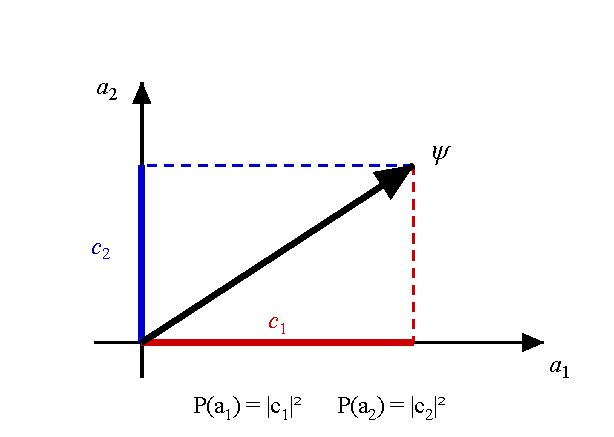
\includegraphics[width=0.56\linewidth]{Capitulo 4/Figuras/MedidaProyeccion.pdf}
            \caption{Contenido geométrico de la regla de Born. El estado se descompone en la base propia del observable y la probabilidad de cada resultado es el cuadrado del módulo de la componente correspondiente.}
            \label{fig:MedidaProyeccion}
        \end{figure}

        La prescripción es consistente, es decir, las probabilidades suman uno. Sumando \eqref{eq:ReglaBorn} sobre todos los resultados posibles y usando la completitud de la base de vectores propios,
        \begin{equation}\label{eq:SumaProbabilidades}
            \sum_{n}P(a_{n}) = \sum_{n}\braket{\psi|\hat{P}_{n}|\psi} = \braket{\psi|\left(\sum_{n}\hat{P}_{n}\right)|\psi} = \braket{\psi|\hat{\mathbb{1}}|\psi} = \braket{\psi|\psi} = 1,
        \end{equation}
        donde el último paso usa la normalización exigida en el postulado \ref{sup:Estado}. La normalización del estado y la conservación de la probabilidad son, por tanto, la misma condición, y esa es la razón de que el primer postulado exija norma unidad.

        De la regla de Born se sigue de inmediato la expresión del valor medio de una magnitud, que es la cantidad que efectivamente se compara con el experimento cuando la medida se repite muchas veces sobre sistemas preparados de manera idéntica. Por definición de promedio estadístico,
        \begin{equation}\label{eq:ValorMedio1}
            \left\langle A\right\rangle = \sum_{n} a_{n}P(a_{n}) = \sum_{n}a_{n}\braket{\psi|\hat{P}_{n}|\psi} = \braket{\psi|\left(\sum_{n}a_{n}\hat{P}_{n}\right)|\psi},
        \end{equation}
        y reconociendo en el paréntesis la descomposición espectral \eqref{eq:DescomposicionEspectral} del propio operador obtenemos la fórmula fundamental
        \begin{equation}\label{eq:ValorMedio}
            \boxed{\;\left\langle A\right\rangle_{\psi} = \braket{\psi|\hat{A}|\psi} .\;}
        \end{equation}
        Este resultado no es un postulado adicional sino una consecuencia de \eqref{eq:ReglaBorn}, y hay que tenerlo presente porque en muchos textos se enuncia como si fuese independiente.

        La segunda parte del postulado, la proyección del estado tras la medida, es con mucho la más problemática de toda la teoría y sería deshonesto presentarla sin señalarlo. Su justificación operativa es sólida: si medimos dos veces seguidas la misma magnitud sin dar tiempo al sistema a evolucionar, obtenemos el mismo resultado, y la única manera de que la teoría reproduzca ese hecho experimental es que la primera medida haya dejado al sistema en el estado propio correspondiente. En efecto, aplicando \eqref{eq:ReglaBorn} al estado proyectado,
        \begin{equation}\label{eq:MedidaRepetida}
            P'(a_{m}) = \frac{\braket{\psi|\hat{P}_{n}\hat{P}_{m}\hat{P}_{n}|\psi}}{\braket{\psi|\hat{P}_{n}|\psi}} = \frac{\delta_{nm}\braket{\psi|\hat{P}_{n}|\psi}}{\braket{\psi|\hat{P}_{n}|\psi}} = \delta_{nm},
        \end{equation}
        donde hemos usado la ortogonalidad de los proyectores, de manera que el segundo resultado coincide con el primero con certeza.

        La dificultad es de otro orden y es la siguiente. El cuarto postulado, que enunciaremos a continuación, afirma que la evolución de un sistema aislado es unitaria, y por tanto lineal, determinista y reversible; el tercero afirma que la medida produce un salto no lineal, indeterminista e irreversible. Un aparato de medida está hecho de átomos y debería obedecer al cuarto postulado, de modo que la teoría contiene dos leyes de evolución incompatibles y no especifica dónde está la frontera entre sus dominios de aplicación. Esta es la formulación precisa del llamado \textit{problema de la medida}, y no está resuelto. Las respuestas que se han propuesto van desde negar que el colapso sea un proceso físico, como en la interpretación de Copenhague, hasta negar que ocurra en absoluto, como en la interpretación de los muchos mundos, pasando por modificar la ecuación de evolución para que el colapso emerja de ella, como en los modelos de colapso espontáneo. La teoría de la decoherencia explica de manera satisfactoria por qué las superposiciones macroscópicas se vuelven inobservables con enorme rapidez, y ese es un avance genuino, pero no explica por qué de todos los resultados posibles se realiza uno concreto. Que una teoría con esta fisura conceptual sea al mismo tiempo la más precisa jamás construida, con predicciones verificadas hasta la duodécima cifra decimal, es probablemente el hecho más desconcertante de la física contemporánea.

        Cuando el valor propio $a_{n}$ está degenerado, es decir, cuando le corresponde un subespacio de dimensión mayor que uno, la regla de proyección debe formularse con el proyector sobre todo el subespacio y no sobre un vector particular, como estableció Lüders en 1950 \citep{luders1950zustandsanderung}; las expresiones \eqref{eq:ReglaBorn} y \eqref{eq:Colapso} ya están escritas en esa forma general, y por eso hemos preferido escribirlas con proyectores en lugar de con productos escalares.

    \subsection{Cuarto postulado: la evolución}

        \begin{Assumption}[Evolución]\label{sup:Evolucion}
            Entre medidas, el estado de un sistema aislado evoluciona de manera determinista según la ecuación de Schrödinger
            \begin{equation}\label{eq:SchrodingerPostulado}
                i\hbar\frac{d}{dt}\ket{\psi(t)} = \hat{H}\ket{\psi(t)},
            \end{equation}
            donde $\hat{H}$ es el operador hamiltoniano del sistema, obtenido del hamiltoniano clásico mediante la correspondencia canónica.
        \end{Assumption}

        La estructura de esta evolución se entiende mejor introduciendo el \textit{operador de evolución} $\hat{U}(t,t_{0})$ definido por
        \begin{equation}\label{eq:OperadorEvolucion}
            \ket{\psi(t)} = \hat{U}(t,t_{0})\ket{\psi(t_{0})},
        \end{equation}
        que para un hamiltoniano independiente del tiempo se obtiene integrando formalmente \eqref{eq:SchrodingerPostulado},
        \begin{equation}\label{eq:ExponencialEvolucion}
            \hat{U}(t,t_{0}) = \exp\left[-\frac{i}{\hbar}\hat{H}\left(t-t_{0}\right)\right],
        \end{equation}
        donde la exponencial de un operador se define mediante su serie de potencias. Que esta expresión resuelve la ecuación se comprueba derivándola término a término,
        \begin{equation}\label{eq:VerificacionU}
            i\hbar\frac{d\hat{U}}{dt} = i\hbar\left(-\frac{i}{\hbar}\hat{H}\right)\exp\left[-\frac{i}{\hbar}\hat{H}(t-t_{0})\right] = \hat{H}\hat{U},
        \end{equation}
        donde el producto $i\hbar\cdot(-i/\hbar) = 1$ deja exactamente el hamiltoniano.

        La propiedad esencial de esta evolución es su unitariedad, que demostramos a continuación porque es el fundamento de la conservación de la probabilidad.

        \begin{myteo}\label{teo:Unitariedad}
            Si $\hat{H}$ es autoadjunto, entonces el operador de evolución satisface $\hat{U}^{\dagger}\hat{U} = \hat{U}\hat{U}^{\dagger} = \hat{\mathbb{1}}$, y en consecuencia la norma del estado se conserva.
        \end{myteo}

        \textbf{\textit{Demostración:}} el adjunto de la exponencial se obtiene conjugando la serie término a término, lo que cambia el signo del exponente imaginario y sustituye $\hat{H}$ por $\hat{H}^{\dagger}$,
        \begin{equation}\label{eq:AdjuntoU}
            \hat{U}^{\dagger} = \exp\left[+\frac{i}{\hbar}\hat{H}^{\dagger}\left(t-t_{0}\right)\right] = \exp\left[+\frac{i}{\hbar}\hat{H}\left(t-t_{0}\right)\right],
        \end{equation}
        donde el segundo paso usa la hipótesis $\hat{H}^{\dagger} = \hat{H}$. Multiplicando ambos operadores, y teniendo en cuenta que las exponenciales de un mismo operador conmutan entre sí, de manera que sus exponentes se suman,
        \begin{equation}\label{eq:ProductoU}
            \hat{U}^{\dagger}\hat{U} = \exp\left[\textcolor{red}{+\frac{i}{\hbar}\hat{H}(t-t_{0})} \textcolor{red}{-\frac{i}{\hbar}\hat{H}(t-t_{0})}\right] = \exp\left(0\right) = \hat{\mathbb{1}},
        \end{equation}
        donde los dos exponentes marcados en rojo se cancelan idénticamente. La conservación de la norma se sigue de inmediato,
        \begin{equation}\label{eq:ConservacionNorma}
            \braket{\psi(t)|\psi(t)} = \braket{\psi(t_{0})|\hat{U}^{\dagger}\hat{U}|\psi(t_{0})} = \braket{\psi(t_{0})|\psi(t_{0})} = 1 . \qquad\blacksquare
        \end{equation}

        La lectura física de este teorema es que la autoadjunción del hamiltoniano, que ya habíamos exigido por ser la energía un observable, garantiza además que la probabilidad total no se pierda durante la evolución. Un hamiltoniano no autoadjunto describiría un sistema en el cual las partículas desaparecen, y de hecho los hamiltonianos efectivos no hermíticos se usan deliberadamente en óptica para describir medios con pérdidas, donde los fotones son absorbidos y la probabilidad de detectarlos efectivamente disminuye.

        Hay además una relación entre este postulado y el capítulo anterior. Comparando \eqref{eq:ExponencialEvolucion} con el propagador \eqref{eq:DefinicionPropagador} que definimos allí vemos que el núcleo de Feynman no es otra cosa que el elemento de matriz del operador de evolución entre estados de posición,
        \begin{equation}\label{eq:PropagadorComoU}
            K(x_{F},t;x_{I},0) = \braket{x_{F}|\hat{U}(t,0)|x_{I}},
        \end{equation}
        de modo que la integral de camino \eqref{eq:IntegralCamino} es una manera de calcular la exponencial de un operador sumando sobre trayectorias clásicas. Los dos formalismos son equivalentes y usaremos uno u otro según convenga.

    \subsection{Quinto postulado: sistemas compuestos}

        \begin{Assumption}[Composición]\label{sup:Composicion}
            El espacio de estados de un sistema compuesto por dos subsistemas $A$ y $B$ es el producto tensorial de los espacios de cada uno,
            \begin{equation}\label{eq:ProductoTensorial}
                \mathcal{H}_{AB} = \mathcal{H}_{A}\otimes\mathcal{H}_{B} .
            \end{equation}
        \end{Assumption}

        Si $\{\ket{a_{i}}\}$ y $\{\ket{b_{j}}\}$ son bases de cada factor, entonces $\{\ket{a_{i}}\otimes\ket{b_{j}}\}$ es una base del conjunto, de manera que la dimensión del espacio compuesto es el \textit{producto} de las dimensiones y no su suma, como ocurriría en una suma directa. Esa diferencia, que parece puramente aritmética, tiene una consecuencia física enorme: el estado más general del sistema compuesto,
        \begin{equation}\label{eq:EstadoCompuesto}
            \ket{\Psi} = \sum_{i,j}c_{ij}\,\ket{a_{i}}\otimes\ket{b_{j}},
        \end{equation}
        no puede en general factorizarse en la forma $\ket{\psi_{A}}\otimes\ket{\psi_{B}}$, pues para que ello ocurra la matriz de coeficientes $c_{ij}$ debe tener rango uno, condición que la inmensa mayoría de las matrices no cumple. Los estados que no admiten esa factorización se llaman \textit{entrelazados}, y son la regla y no la excepción.

        Merece la pena detenerse en lo que acaba de aparecer, porque no es un tecnicismo del producto tensorial. La existencia de estados entrelazados es la consecuencia más profunda del formalismo y la que separa de manera más nítida a la física cuántica de la clásica, porque en un estado entrelazado el sistema compuesto está en un estado puro, es decir, perfectamente determinado, mientras que ninguno de sus subsistemas lo está. El todo está mejor definido que las partes, afirmación que no tiene ningún análogo clásico posible. Para describir el estado de uno solo de los subsistemas necesitaremos la matriz densidad, que introduciremos al final del capítulo, y que es precisamente el objeto que la teoría exige cuando se renuncia a mirar el sistema completo.

\section{Compatibilidad y el principio de indeterminación}

        El hecho de que los observables sean operadores, y de que los operadores en general no conmuten, introduce en la física una restricción que no tiene contrapartida clásica: no todas las magnitudes pueden determinarse simultáneamente. El resultado preciso es el siguiente.

        \begin{myteo}\label{teo:Compatibles}
            Dos observables $\hat{A}$ y $\hat{B}$ admiten un conjunto completo de vectores propios comunes si y solo si conmutan, $[\hat{A},\hat{B}] = 0$.
        \end{myteo}

        \textbf{\textit{Demostración:}} supongamos primero que existe una base común $\{\ket{n}\}$ tal que $\hat{A}\ket{n} = a_{n}\ket{n}$ y $\hat{B}\ket{n} = b_{n}\ket{n}$. Aplicando el conmutador a cualquier elemento de la base,
        \begin{equation}\label{eq:ConmutadorBase}
            \left[\hat{A},\hat{B}\right]\ket{n} = \hat{A}\hat{B}\ket{n} - \hat{B}\hat{A}\ket{n} = b_{n}\hat{A}\ket{n} - a_{n}\hat{B}\ket{n} = \left(\textcolor{red}{a_{n}b_{n}} - \textcolor{red}{b_{n}a_{n}}\right)\ket{n} = 0,
        \end{equation}
        donde los dos productos marcados en rojo se cancelan por ser números y conmutar entre sí. Como el conmutador anula a todos los elementos de una base, y es lineal, anula a todo el espacio y por tanto es el operador nulo.

        Recíprocamente, supongamos $[\hat{A},\hat{B}] = 0$ y sea $\ket{a}$ un vector propio de $\hat{A}$ con valor propio $a$ no degenerado. Entonces
        \begin{equation}\label{eq:ReciprocoConmutan}
            \hat{A}\left(\hat{B}\ket{a}\right) = \hat{B}\hat{A}\ket{a} = a\left(\hat{B}\ket{a}\right),
        \end{equation}
        donde el primer paso usa la conmutación. La igualdad afirma que el vector $\hat{B}\ket{a}$ es también vector propio de $\hat{A}$ con el mismo valor propio $a$, y como hemos supuesto que ese valor propio no está degenerado, el subespacio correspondiente tiene dimensión uno y por tanto $\hat{B}\ket{a}$ debe ser proporcional a $\ket{a}$,
        \begin{equation}\label{eq:BEsPropio}
            \hat{B}\ket{a} = b\ket{a},
        \end{equation}
        es decir, $\ket{a}$ es también vector propio de $\hat{B}$. Cuando hay degeneración el argumento se aplica dentro de cada subespacio propio de $\hat{A}$, donde $\hat{B}$ actúa como un operador autoadjunto y puede diagonalizarse por el teorema espectral. $\blacksquare$

        La interpretación física es directa, pero hay que enunciarla con cuidado, porque se presta a confusión. Si dos observables conmutan, existe una base de estados en los cuales ambos tienen valor definido, y medir uno no perturba el valor del otro, de modo que pueden medirse en cualquier orden con resultados reproducibles; se dice entonces que son \textit{compatibles}. Si no conmutan, no existe tal base, y la afirmación de que el sistema posee simultáneamente valores definidos de ambas magnitudes carece de sentido dentro de la teoría. No se trata de que el sistema tenga esos valores y nosotros no podamos conocerlos, sino de que la teoría no le atribuye tales valores, y esta distinción, que Bohr insistió en subrayar durante toda su vida, es la diferencia entre la mecánica cuántica y una teoría clásica con ignorancia añadida.

        Un conjunto de observables que conmutan dos a dos y cuyos valores propios simultáneos identifican unívocamente a cada elemento de la base se llama \textit{conjunto completo de observables compatibles}, y proporciona la manera sistemática de etiquetar los estados de un sistema. En el capítulo siguiente los estados del campo electromagnético en una cavidad se etiquetarán mediante los números de ocupación de todos los modos, que forman precisamente un conjunto de esta clase.

        La incompatibilidad admite una formulación cuantitativa. Definamos la \textit{dispersión} de un observable en un estado dado como la raíz cuadrada de la varianza,
        \begin{equation}\label{eq:Dispersion}
            \left(\Delta A\right)^{2} \equiv \left\langle\left(\hat{A} - \left\langle A\right\rangle\right)^{2}\right\rangle = \left\langle \hat{A}^{2}\right\rangle - \left\langle A\right\rangle^{2},
        \end{equation}
        donde la segunda igualdad se obtiene desarrollando el cuadrado y usando la linealidad del valor medio. La dispersión mide cuánto fluctúan los resultados de la medida alrededor de su promedio, y se anula si y solo si el estado es un vector propio del observable.

        \begin{myteo}[Robertson]\label{teo:Robertson}
            Para cualesquiera dos observables $\hat{A}$ y $\hat{B}$ y cualquier estado normalizado $\ket{\psi}$ se cumple
            \begin{equation}\label{eq:Robertson}
                \Delta A\,\Delta B \;\geq\; \frac{1}{2}\left|\left\langle\left[\hat{A},\hat{B}\right]\right\rangle\right| .
            \end{equation}
        \end{myteo}

        \textbf{\textit{Demostración:}} definamos los operadores centrados
        \begin{equation}\label{eq:OperadoresCentrados}
            \hat{\mathcal{A}} = \hat{A} - \left\langle A\right\rangle, \qquad \hat{\mathcal{B}} = \hat{B} - \left\langle B\right\rangle,
        \end{equation}
        que son autoadjuntos por serlo $\hat{A}$ y $\hat{B}$ y por ser reales sus valores medios, y que satisfacen $\left(\Delta A\right)^{2} = \braket{\psi|\hat{\mathcal{A}}^{2}|\psi}$ y análogamente para $\hat{\mathcal{B}}$. Su conmutador, además, coincide con el de los operadores originales, pues las constantes conmutan con todo,
        \begin{equation}\label{eq:ConmutadorCentrado}
            \left[\hat{\mathcal{A}},\hat{\mathcal{B}}\right] = \left[\hat{A} - \left\langle A\right\rangle,\;\hat{B} - \left\langle B\right\rangle\right] = \left[\hat{A},\hat{B}\right] .
        \end{equation}

        Con los vectores $\ket{u} = \hat{\mathcal{A}}\ket{\psi}$ y $\ket{v} = \hat{\mathcal{B}}\ket{\psi}$, cuyas normas al cuadrado son precisamente las varianzas, se tiene
        \begin{equation}\label{eq:NormasUV}
            \braket{u|u} = \braket{\psi|\hat{\mathcal{A}}^{\dagger}\hat{\mathcal{A}}|\psi} = \braket{\psi|\hat{\mathcal{A}}^{2}|\psi} = \left(\Delta A\right)^{2},
            \qquad
            \braket{v|v} = \left(\Delta B\right)^{2} .
        \end{equation}
        La desigualdad de Cauchy y Schwarz, válida en todo espacio con producto interno, afirma que
        \begin{equation}\label{eq:CauchySchwarz}
            \braket{u|u}\braket{v|v} \geq \left|\braket{u|v}\right|^{2},
        \end{equation}
        de manera que el problema se reduce a acotar inferiormente el miembro derecho. El número complejo $\braket{u|v}$ se separa en sus partes real e imaginaria como
        \begin{equation}\label{eq:SeparacionZ}
            \braket{u|v} = \braket{\psi|\hat{\mathcal{A}}\hat{\mathcal{B}}|\psi} = \frac{1}{2}\braket{\psi|\left\{\hat{\mathcal{A}},\hat{\mathcal{B}}\right\}|\psi} + \frac{1}{2}\braket{\psi|\left[\hat{\mathcal{A}},\hat{\mathcal{B}}\right]|\psi},
        \end{equation}
        donde hemos usado la identidad $\hat{\mathcal{A}}\hat{\mathcal{B}} = \frac{1}{2}\{\hat{\mathcal{A}},\hat{\mathcal{B}}\} + \frac{1}{2}[\hat{\mathcal{A}},\hat{\mathcal{B}}]$, que se comprueba desarrollando el anticonmutador y el conmutador y observando que los términos $\hat{\mathcal{B}}\hat{\mathcal{A}}$ se cancelan,
        \begin{equation}\label{eq:IdentidadAntiConm}
            \frac{1}{2}\left(\hat{\mathcal{A}}\hat{\mathcal{B}} + \textcolor{red}{\hat{\mathcal{B}}\hat{\mathcal{A}}}\right) + \frac{1}{2}\left(\hat{\mathcal{A}}\hat{\mathcal{B}} - \textcolor{red}{\hat{\mathcal{B}}\hat{\mathcal{A}}}\right) = \hat{\mathcal{A}}\hat{\mathcal{B}} .
        \end{equation}

        Los dos términos de \eqref{eq:SeparacionZ} tienen carácter distinto, y esa es la clave de la demostración. El anticonmutador de dos operadores autoadjuntos es autoadjunto, de modo que su valor medio es real; el conmutador de dos operadores autoadjuntos es antiautoadjunto, pues
        \begin{equation}\label{eq:ConmutadorAntihermitico}
            \left[\hat{\mathcal{A}},\hat{\mathcal{B}}\right]^{\dagger} = \left(\hat{\mathcal{A}}\hat{\mathcal{B}}\right)^{\dagger} - \left(\hat{\mathcal{B}}\hat{\mathcal{A}}\right)^{\dagger} = \hat{\mathcal{B}}\hat{\mathcal{A}} - \hat{\mathcal{A}}\hat{\mathcal{B}} = -\left[\hat{\mathcal{A}},\hat{\mathcal{B}}\right],
        \end{equation}
        y el valor medio de un operador antiautoadjunto es imaginario puro. El módulo al cuadrado de \eqref{eq:SeparacionZ} es por tanto la suma de los cuadrados de ambas contribuciones,
        \begin{equation}\label{eq:ModuloZ}
            \left|\braket{u|v}\right|^{2} = \frac{1}{4}\left|\left\langle\left\{\hat{\mathcal{A}},\hat{\mathcal{B}}\right\}\right\rangle\right|^{2} + \frac{1}{4}\left|\left\langle\left[\hat{\mathcal{A}},\hat{\mathcal{B}}\right]\right\rangle\right|^{2}
            \;\geq\; \frac{1}{4}\left|\left\langle\left[\hat{\mathcal{A}},\hat{\mathcal{B}}\right]\right\rangle\right|^{2},
        \end{equation}
        donde la desigualdad final se obtiene simplemente descartando el primer sumando, que es no negativo. Combinando \eqref{eq:NormasUV}, \eqref{eq:CauchySchwarz} y \eqref{eq:ModuloZ}, y usando \eqref{eq:ConmutadorCentrado},
        \begin{equation}\label{eq:RobertsonFinal}
            \left(\Delta A\right)^{2}\left(\Delta B\right)^{2} \geq \frac{1}{4}\left|\left\langle\left[\hat{A},\hat{B}\right]\right\rangle\right|^{2},
        \end{equation}
        y tomando la raíz cuadrada, que preserva la desigualdad por ser ambos miembros no negativos, se obtiene \eqref{eq:Robertson}. $\blacksquare$

        Aplicando el teorema al par canónico, cuyo conmutador es el número $i\hbar$ según \eqref{eq:ConmutadorHistorico}, el valor medio se calcula de inmediato porque una constante sale fuera y el estado está normalizado,
        \begin{equation}\label{eq:HeisenbergCanonico}
            \Delta x\,\Delta p \geq \frac{1}{2}\left|\braket{\psi|i\hbar|\psi}\right| = \frac{\hbar}{2}\left|\braket{\psi|\psi}\right| = \frac{\hbar}{2},
        \end{equation}
        que es la relación de indeterminación de Heisenberg en la forma precisa que le dio Kennard \citep{kennard1927quantenmechanik}.

        La interpretación de \eqref{eq:HeisenbergCanonico} exige cuidado porque la que popularizó Heisenberg es incorrecta, o al menos gravemente incompleta. El argumento del microscopio de rayos gamma, según el cual al iluminar el electrón con un fotón de longitud de onda corta se le transfiere un momento incontrolado, describe un efecto real pero sugiere que la partícula \textit{tiene} una posición y un momento definidos que la medida perturba. Nada en la demostración anterior se refiere a perturbación alguna: la desigualdad \eqref{eq:Robertson} es una propiedad del estado, no del procedimiento de medida, y afirma que \textbf{no existe ningún estado en el cual ambas dispersiones sean simultáneamente arbitrariamente pequeñas}. Las dispersiones se determinan midiendo cada magnitud sobre sistemas distintos preparados de manera idéntica, de modo que ni siquiera hace falta medir ambas sobre el mismo sistema para que la relación se manifieste. La indeterminación es una propiedad de la preparación y no del acto de medir.

        Vale la pena añadir, porque lo usaremos en el capítulo siguiente, que la desigualdad \eqref{eq:HeisenbergCanonico} se satura, es decir, se convierte en igualdad, precisamente para los estados gaussianos, y que en el contexto del campo electromagnético esa saturación define a los estados coherentes y, cuando además se redistribuye la incertidumbre entre las dos cuadraturas, a los estados comprimidos. La luz comprimida consiste en explotar el hecho de que \eqref{eq:HeisenbergCanonico} acota el producto de las dispersiones y no cada una de ellas por separado, de manera que una cuadratura puede medirse con precisión arbitraria a costa de la otra.

\section{Representaciones}

        El formalismo desarrollado hasta aquí es abstracto, en el sentido de que no hace referencia a ninguna base concreta. Para calcular hay que escoger una, y las dos elecciones habituales son las bases de vectores propios de la posición y del momento.

        En la \textit{representación de posición} se desarrolla el estado en la base $\{\ket{x}\}$ mediante la completitud continua \eqref{eq:CompletitudContinua},
        \begin{equation}\label{eq:FuncionOnda}
            \ket{\psi} = \int_{\mathbb{R}}\ket{x}\braket{x|\psi}\,dx \equiv \int_{\mathbb{R}}\psi(x)\ket{x}\,dx,
            \qquad
            \psi(x) \equiv \braket{x|\psi},
        \end{equation}
        y la colección de coeficientes $\psi(x)$ es precisamente la \textit{función de onda} de Schrödinger. La función de onda no es el estado sino sus componentes en una base particular, exactamente como las tres componentes de un vector ordinario no son el vector sino su expresión en unos ejes escogidos, y esta observación, evidente una vez formulada, es la que disuelve la pretendida rivalidad entre la mecánica ondulatoria y la matricial.

        En esta representación la regla de Born \eqref{eq:ReglaBorn} adopta la forma familiar: la probabilidad de hallar la partícula en el intervalo $[x,x+dx]$ es
        \begin{equation}\label{eq:BornPosicion}
            dP = \left|\braket{x|\psi}\right|^{2}dx = \left|\psi(x)\right|^{2}dx,
        \end{equation}
        que es la interpretación que Born propuso en su nota al pie de 1926 \citep{born1926stossvorgange}.

        La acción del operador de posición es multiplicativa, pues $\braket{x|\hat{x}|\psi} = x\braket{x|\psi} = x\psi(x)$. Para el operador de momento la acción se deduce del conmutador canónico, y hacemos el cálculo porque suele presentarse como una definición cuando en realidad es un teorema. Partiendo de la identidad $[\hat{x},\hat{p}] = i\hbar$ y tomando su elemento de matriz entre estados de posición,
        \begin{equation}\label{eq:ElementoConmutador}
            \braket{x|\left(\hat{x}\hat{p} - \hat{p}\hat{x}\right)|x'} = \left(x - x'\right)\braket{x|\hat{p}|x'} = i\hbar\,\delta\left(x-x'\right),
        \end{equation}
        donde hemos dejado actuar $\hat{x}$ hacia la izquierda en el primer término y hacia la derecha en el segundo, lo que es lícito por ser autoadjunto. La solución de esta ecuación, en el sentido de las distribuciones, es
        \begin{equation}\label{eq:MomentoDistribucion}
            \braket{x|\hat{p}|x'} = -i\hbar\,\frac{\partial}{\partial x}\delta\left(x-x'\right),
        \end{equation}
        como se verifica usando la propiedad $y\,\delta'(y) = -\delta(y)$ de la delta de Dirac. Aplicando \eqref{eq:MomentoDistribucion} a un estado arbitrario e integrando por partes,
        \begin{equation}\label{eq:MomentoDerivada}
            \braket{x|\hat{p}|\psi} = \int_{\mathbb{R}}\braket{x|\hat{p}|x'}\braket{x'|\psi}dx'
            = -i\hbar\int_{\mathbb{R}}\frac{\partial\delta(x-x')}{\partial x}\psi(x')\,dx'
            = -i\hbar\frac{\partial\psi(x)}{\partial x},
        \end{equation}
        de manera que en la representación de posición el momento actúa como una derivada,
        \begin{equation}\label{eq:OperadorMomento}
            \boxed{\;\hat{p} \;\longrightarrow\; -i\hbar\frac{\partial}{\partial x} .\;}
        \end{equation}
        Sustituyendo esta prescripción y la multiplicativa para la posición en el hamiltoniano $\hat{H} = \hat{p}^{2}/2m + V(\hat{x})$, la ecuación de evolución \eqref{eq:SchrodingerPostulado} se convierte literalmente en la ecuación diferencial \eqref{eq:SchrodingerTemporal} que dedujimos en el capítulo anterior siguiendo el razonamiento de Schrödinger. Aquel camino, que partía de la óptica y de Hamilton-Jacobi, y este, que parte de los postulados y del álgebra de conmutadores, conducen exactamente a la misma ecuación.

        La relación entre las dos representaciones es de especial interés en este libro, porque resulta ser la misma transformación que gobierna la difracción en campo lejano estudiada en el capítulo primero.

        Los estados propios del momento en la representación de posición se obtienen resolviendo la ecuación de valores propios $\hat{p}\ket{p} = p\ket{p}$ con la prescripción \eqref{eq:OperadorMomento},
        \begin{equation}\label{eq:EcuacionPropiosP}
            -i\hbar\frac{\partial}{\partial x}\braket{x|p} = p\braket{x|p},
        \end{equation}
        que es una ecuación diferencial ordinaria de primer orden cuya solución es una exponencial. Separando variables e integrando,
        \begin{equation}\label{eq:SolucionPropiosP}
            \frac{\partial\braket{x|p}}{\braket{x|p}} = \frac{ip}{\hbar}\partial x
            \qquad\Longrightarrow\qquad
            \braket{x|p} = \frac{1}{\sqrt{2\pi\hbar}}\,e^{ipx/\hbar},
        \end{equation}
        donde la constante de normalización se fija exigiendo $\braket{p|p'} = \delta(p-p')$ y usando la representación integral de la delta. Estas son ondas planas, es decir, exactamente los objetos que en el capítulo primero describían la propagación de una componente espectral del campo.

        Insertando la completitud en posiciones, la función de onda en la representación de momentos resulta ser
        \begin{equation}\label{eq:FourierMomento}
            \tilde{\psi}(p) = \braket{p|\psi} = \int_{\mathbb{R}}\braket{p|x}\braket{x|\psi}\,dx
            = \frac{1}{\sqrt{2\pi\hbar}}\int_{\mathbb{R}}\psi(x)\,e^{-ipx/\hbar}\,dx,
        \end{equation}
        que es la transformada de Fourier de la función de onda, con $\hbar$ haciendo el papel de la constante que empareja las dos variables conjugadas. Posición y momento son variables conjugadas de Fourier, del mismo modo que lo son la coordenada en el plano del objeto y la frecuencia espacial en el plano de Fraunhofer, y esa coincidencia explica por qué el principio de indeterminación tiene un análogo exacto en óptica clásica: el producto de la anchura de una abertura por la anchura angular de su patrón de difracción está acotado inferiormente por la misma razón matemática por la cual lo está $\Delta x\,\Delta p$. En ambos casos se trata del teorema según el cual una función y su transformada de Fourier no pueden estar ambas arbitrariamente concentradas.

        La conexión llega aún más lejos. En el capítulo primero demostramos que la propagación de Fresnel entre dos superficies esféricas es una transformada fraccionaria de Fourier, es decir, una interpolación continua entre la identidad y la transformada ordinaria. En el capítulo anterior obtuvimos que la evolución temporal de un oscilador armónico es esa misma transformación, con el ángulo fraccionario igual a $\omega t$. Y ahora vemos que la transformada ordinaria conecta las representaciones de posición y momento. Las tres afirmaciones son consistentes entre sí y dicen, reunidas, que la evolución de un oscilador armónico durante un cuarto de período intercambia exactamente los papeles de la posición y del momento, hecho que en el capítulo siguiente reaparecerá como la rotación de las cuadraturas del campo electromagnético en el espacio de fase.

\section{Las imágenes de evolución}

        El postulado \ref{sup:Evolucion} atribuye la evolución temporal al estado y deja fijos los operadores, y esa es la llamada \textit{imagen de Schrödinger}. Sin embargo, todo lo que la teoría predice son valores medios de la forma \eqref{eq:ValorMedio}, y en esa expresión aparecen tanto el estado como el operador, de manera que la asignación de la dependencia temporal a uno u otro es convencional. Podemos escribir el valor medio en el instante $t$ sustituyendo la evolución \eqref{eq:OperadorEvolucion},
        \begin{equation}\label{eq:ValorMedioEvolucionado}
            \left\langle A\right\rangle_{t} = \braket{\psi(t)|\hat{A}|\psi(t)}
            = \braket{\psi(0)|\hat{U}^{\dagger}(t)\,\hat{A}\,\hat{U}(t)|\psi(0)},
        \end{equation}
        y observemos que la misma expresión admite dos lecturas: podemos agrupar los operadores de evolución con los estados, que es la imagen de Schrödinger, o agruparlos con el observable, definiendo
        \begin{equation}\label{eq:OperadorHeisenberg}
            \hat{A}_{H}(t) \equiv \hat{U}^{\dagger}(t)\,\hat{A}\,\hat{U}(t),
        \end{equation}
        con lo cual el estado permanece congelado y es el operador el que evoluciona. Esta es la \textit{imagen de Heisenberg}, y es literalmente la formulación que Heisenberg construyó en 1925, antes de que existiese la función de onda.

        La ecuación de movimiento de estos operadores se deduce sin dificultad. Derivando \eqref{eq:OperadorHeisenberg} respecto del tiempo mediante la regla del producto, y usando que $d\hat{U}/dt = -i\hat{H}\hat{U}/\hbar$ junto con su adjunta $d\hat{U}^{\dagger}/dt = +i\hat{U}^{\dagger}\hat{H}/\hbar$,
        \begin{equation}\label{eq:DerivadaHeisenberg}
            \frac{d\hat{A}_{H}}{dt} = \frac{i}{\hbar}\hat{U}^{\dagger}\hat{H}\hat{A}\hat{U} - \frac{i}{\hbar}\hat{U}^{\dagger}\hat{A}\hat{H}\hat{U} + \hat{U}^{\dagger}\frac{\partial\hat{A}}{\partial t}\hat{U},
        \end{equation}
        donde el último término recoge una posible dependencia temporal explícita del observable. Insertando la identidad $\hat{U}\hat{U}^{\dagger} = \hat{\mathbb{1}}$ entre los operadores de cada producto, lo que es lícito por la unitariedad demostrada en el teorema \ref{teo:Unitariedad}, y reconociendo en cada factor la definición \eqref{eq:OperadorHeisenberg},
        \begin{equation}\label{eq:EcuacionHeisenberg}
            \boxed{\;\frac{d\hat{A}_{H}}{dt} = \frac{1}{i\hbar}\left[\hat{A}_{H},\hat{H}\right] + \left(\frac{\partial\hat{A}}{\partial t}\right)_{H} .\;}
        \end{equation}

        Al lado de esta ecuación vale la pena poner la ecuación de movimiento clásica en forma de Poisson que obtuvimos en el capítulo anterior,
        \begin{equation}\label{eq:ComparacionPoisson}
            \frac{df}{dt} = \left\{f,H\right\} + \frac{\partial f}{\partial t},
        \end{equation}
        y la correspondencia es exacta bajo la regla de Dirac \eqref{eq:CorrespondenciaDirac}, que sustituye el corchete de Poisson por el conmutador dividido por $i\hbar$. La imagen de Heisenberg es la mecánica hamiltoniana con los observables convertidos en operadores y el corchete de Poisson convertido en conmutador, y esa identidad estructural es la razón por la cual el procedimiento de cuantización canónica funciona. En el capítulo siguiente aplicaremos \eqref{eq:EcuacionHeisenberg} a los operadores de creación y aniquilación del campo para obtener su dependencia temporal, y comprobaremos que reproduce las oscilaciones armónicas del campo clásico.

    \subsection{El teorema de Ehrenfest y el límite clásico}

        La imagen de Heisenberg permite demostrar con muy poco esfuerzo en qué sentido preciso la mecánica clásica emerge de la cuántica, resultado que Ehrenfest estableció en 1927 \citep{ehrenfest1927bemerkung}.

        Podemos aplicar \eqref{eq:EcuacionHeisenberg} a los operadores canónicos para una partícula con hamiltoniano $\hat{H} = \hat{p}^{2}/2m + V(\hat{x})$. Para la posición necesitamos el conmutador $[\hat{x},\hat{p}^{2}]$, que calculamos insertando el conmutador canónico dos veces,
        \begin{equation}\label{eq:ConmutadorXP2}
            \left[\hat{x},\hat{p}^{2}\right] = \hat{p}\left[\hat{x},\hat{p}\right] + \left[\hat{x},\hat{p}\right]\hat{p} = i\hbar\hat{p} + i\hbar\hat{p} = 2i\hbar\hat{p},
        \end{equation}
        donde hemos usado la identidad $[\hat{A},\hat{B}\hat{C}] = \hat{B}[\hat{A},\hat{C}] + [\hat{A},\hat{B}]\hat{C}$. Sustituyendo en la ecuación de Heisenberg, y teniendo en cuenta que $\hat{x}$ conmuta con $V(\hat{x})$,
        \begin{equation}\label{eq:EhrenfestX}
            \frac{d\hat{x}}{dt} = \frac{1}{i\hbar}\cdot\frac{2i\hbar\hat{p}}{2m} = \frac{\hat{p}}{m} .
        \end{equation}
        Para el momento necesitamos $[\hat{p},V(\hat{x})]$, que se obtiene aplicando la representación \eqref{eq:OperadorMomento} a un estado arbitrario y usando la regla del producto,
        \begin{equation}\label{eq:ConmutadorPV}
            \left[\hat{p},V\right]\psi = -i\hbar\frac{\partial}{\partial x}\left(V\psi\right) + i\hbar V\frac{\partial\psi}{\partial x}
            = -i\hbar\frac{\partial V}{\partial x}\psi - \textcolor{red}{i\hbar V\frac{\partial\psi}{\partial x}} + \textcolor{red}{i\hbar V\frac{\partial\psi}{\partial x}}
            = -i\hbar\frac{\partial V}{\partial x}\psi,
        \end{equation}
        donde los dos términos en rojo se cancelan, de manera que
        \begin{equation}\label{eq:EhrenfestP}
            \frac{d\hat{p}}{dt} = \frac{1}{i\hbar}\left(-i\hbar\frac{\partial V}{\partial x}\right) = -\frac{\partial V}{\partial \hat{x}} .
        \end{equation}
        Tomando valores medios en ambas ecuaciones obtenemos el \textit{teorema de Ehrenfest},
        \begin{equation}\label{eq:Ehrenfest}
            \frac{d\left\langle x\right\rangle}{dt} = \frac{\left\langle p\right\rangle}{m},
            \qquad
            \frac{d\left\langle p\right\rangle}{dt} = -\left\langle\frac{\partial V}{\partial x}\right\rangle,
        \end{equation}
        que son formalmente las ecuaciones de Hamilton \eqref{eq:Hamilton} del capítulo anterior escritas para los valores medios.

        La lectura ingenua de \eqref{eq:Ehrenfest} afirma que los centroides de los paquetes de ondas siguen trayectorias clásicas, y esa lectura es incorrecta en general. La razón está en el segundo miembro de la segunda ecuación: lo que aparece es el valor medio de la derivada del potencial y no la derivada del potencial evaluada en el valor medio,
        \begin{equation}\label{eq:EhrenfestObjecion}
            \left\langle\frac{\partial V}{\partial x}(\hat{x})\right\rangle \neq \frac{\partial V}{\partial x}\left(\left\langle x\right\rangle\right)
            \qquad\text{en general},
        \end{equation}
        y ambas cantidades coinciden únicamente cuando el potencial es a lo sumo cuadrático, en cuyo caso su derivada es lineal y el promedio de una función lineal es la función del promedio, o bien cuando el paquete es tan estrecho que el potencial puede considerarse lineal en su interior. El límite clásico no consiste en que los promedios cuánticos obedezcan ecuaciones clásicas, que es lo que \eqref{eq:Ehrenfest} dice, sino en que además el paquete permanezca estrecho durante el tiempo de interés, condición que falla con rapidez en sistemas caóticos y que se cumple espléndidamente para el oscilador armónico, cuyo potencial es exactamente cuadrático. Este es el mismo mensaje que obtuvimos en el capítulo anterior al examinar el término $i\hbar\nabla^{2}\mathcal{S}/2m$ de la ecuación \eqref{eq:HJCuantica}, escrito ahora en el lenguaje de los operadores.

        Existe una tercera posibilidad, intermedia entre las dos anteriores, que resulta indispensable cuando el hamiltoniano se descompone en una parte libre soluble y una interacción que se desea tratar perturbativamente,
        \begin{equation}\label{eq:HamiltonianoDividido}
            \hat{H} = \hat{H}_{0} + \hat{V} .
        \end{equation}
        En la \textit{imagen de interacción} se atribuye a los operadores la evolución generada por la parte libre y a los estados la generada por la interacción, definiendo
        \begin{equation}\label{eq:ImagenInteraccion}
            \ket{\psi_{I}(t)} = e^{i\hat{H}_{0}t/\hbar}\ket{\psi_{S}(t)},
            \qquad
            \hat{A}_{I}(t) = e^{i\hat{H}_{0}t/\hbar}\,\hat{A}_{S}\,e^{-i\hat{H}_{0}t/\hbar} .
        \end{equation}
        Derivando la primera de estas relaciones respecto del tiempo mediante la regla del producto y sustituyendo la ecuación de Schrödinger,
        \begin{equation}\label{eq:EcuacionInteraccion1}
            i\hbar\frac{d\ket{\psi_{I}}}{dt} = -\hat{H}_{0}e^{i\hat{H}_{0}t/\hbar}\ket{\psi_{S}} + e^{i\hat{H}_{0}t/\hbar}\left(\hat{H}_{0}+\hat{V}\right)\ket{\psi_{S}},
        \end{equation}
        y como $\hat{H}_{0}$ conmuta con su propia exponencial, los dos términos que lo contienen se cancelan,
        \begin{equation}\label{eq:EcuacionInteraccion2}
            i\hbar\frac{d\ket{\psi_{I}}}{dt} = \textcolor{red}{-\hat{H}_{0}e^{i\hat{H}_{0}t/\hbar}\ket{\psi_{S}}} + \textcolor{red}{\hat{H}_{0}e^{i\hat{H}_{0}t/\hbar}\ket{\psi_{S}}} + \hat{V}_{I}(t)\ket{\psi_{I}(t)} = \hat{V}_{I}(t)\ket{\psi_{I}(t)},
        \end{equation}
        de manera que el estado evoluciona únicamente bajo la interacción, expresada en la imagen. Toda la dinámica trivial del sistema libre ha sido absorbida en la definición de los operadores, y lo que queda es exactamente el efecto que interesa calcular. Esta es la imagen en la que se desarrolla la teoría de perturbaciones dependiente del tiempo, la regla de oro de Fermi y el modelo de Jaynes y Cummings para la interacción entre un átomo de dos niveles y un modo del campo, que es el modelo fundamental de la óptica cuántica.

\section{El oscilador armónico en forma algebraica}

    Dedicamos una sección propia al oscilador armónico porque es, sin exageración, el sistema central de toda la óptica cuántica: en el capítulo siguiente demostraremos que el campo electromagnético en una cavidad es dinámicamente equivalente a una colección infinita de osciladores independientes, uno por cada modo, de manera que todo cuanto sepamos resolver aquí se traducirá allí sin esfuerzo. Lo resolveremos por el método algebraico de Dirac, que no requiere resolver ninguna ecuación diferencial y que exhibe con total claridad el origen de la cuantización.

        Partimos del hamiltoniano
        \begin{equation}\label{eq:HamiltonianoOscQ}
            \hat{H} = \frac{\hat{p}^{2}}{2m} + \frac{1}{2}m\omega^{2}\hat{x}^{2},
            \qquad
            \left[\hat{x},\hat{p}\right] = i\hbar,
        \end{equation}
        y observamos que, si los operadores fuesen números, la expresión sería una suma de cuadrados y podría factorizarse como el producto de dos factores conjugados. Intentemos esa factorización y veamos qué impide que sea exacta. Definimos el \textit{operador de aniquilación}
        \begin{equation}\label{eq:DefinicionA}
            \hat{a} \equiv \sqrt{\frac{m\omega}{2\hbar}}\left(\hat{x} + \frac{i}{m\omega}\hat{p}\right),
        \end{equation}
        cuyo adjunto, el \textit{operador de creación}, se obtiene conjugando y recordando que $\hat{x}$ y $\hat{p}$ son autoadjuntos,
        \begin{equation}\label{eq:DefinicionADaga}
            \hat{a}^{\dagger} = \sqrt{\frac{m\omega}{2\hbar}}\left(\hat{x} - \frac{i}{m\omega}\hat{p}\right).
        \end{equation}
        Obsérvese que $\hat{a}$ no es autoadjunto y por tanto no es un observable; es una combinación auxiliar cuya única justificación, por ahora, es que simplifica el álgebra.

        Su conmutador se obtiene desarrollando el producto y usando la bilinealidad,
        \begin{equation}\label{eq:ConmutadorAADaga1}
            \left[\hat{a},\hat{a}^{\dagger}\right] = \frac{m\omega}{2\hbar}\left[\hat{x}+\frac{i\hat{p}}{m\omega},\;\hat{x}-\frac{i\hat{p}}{m\omega}\right]
            = \frac{m\omega}{2\hbar}\left(\textcolor{red}{\left[\hat{x},\hat{x}\right]} - \frac{i}{m\omega}\left[\hat{x},\hat{p}\right] + \frac{i}{m\omega}\left[\hat{p},\hat{x}\right] + \textcolor{red}{\frac{1}{m^{2}\omega^{2}}\left[\hat{p},\hat{p}\right]}\right),
        \end{equation}
        donde los dos conmutadores marcados en rojo se anulan por conmutar todo operador consigo mismo. Usando $[\hat{x},\hat{p}] = i\hbar$ y $[\hat{p},\hat{x}] = -i\hbar$, los dos términos supervivientes resultan iguales y se suman,
        \begin{equation}\label{eq:ConmutadorAADaga2}
            \left[\hat{a},\hat{a}^{\dagger}\right] = \frac{m\omega}{2\hbar}\left(-\frac{i}{m\omega}\cdot i\hbar - \frac{i}{m\omega}\cdot i\hbar\right)
            = \frac{m\omega}{2\hbar}\cdot\frac{2\hbar}{m\omega} = 1 .
        \end{equation}
        La relación $\left[\hat{a},\hat{a}^{\dagger}\right] = 1$ es toda el álgebra que necesitaremos, y es equivalente al conmutador canónico: contiene exactamente la misma información escrita en otras variables.

        Invirtiendo \eqref{eq:DefinicionA} y \eqref{eq:DefinicionADaga}, es decir, sumando y restando ambas expresiones, se recuperan las variables originales,
        \begin{equation}\label{eq:XPenA}
            \hat{x} = \sqrt{\frac{\hbar}{2m\omega}}\left(\hat{a}+\hat{a}^{\dagger}\right),
            \qquad
            \hat{p} = -i\sqrt{\frac{m\omega\hbar}{2}}\left(\hat{a}-\hat{a}^{\dagger}\right).
        \end{equation}
        Sustituyendo en el hamiltoniano \eqref{eq:HamiltonianoOscQ} y desarrollando ambos cuadrados con cuidado de no alterar el orden de los factores, el término cinético da
        \begin{equation}\label{eq:CineticoEnA}
            \frac{\hat{p}^{2}}{2m} = \frac{1}{2m}\left(-\frac{m\omega\hbar}{2}\right)\left(\hat{a}-\hat{a}^{\dagger}\right)^{2}
            = -\frac{\hbar\omega}{4}\left(\hat{a}^{2} - \hat{a}\hat{a}^{\dagger} - \hat{a}^{\dagger}\hat{a} + \hat{a}^{\dagger 2}\right),
        \end{equation}
        y el término potencial
        \begin{equation}\label{eq:PotencialEnA}
            \frac{1}{2}m\omega^{2}\hat{x}^{2} = \frac{1}{2}m\omega^{2}\cdot\frac{\hbar}{2m\omega}\left(\hat{a}+\hat{a}^{\dagger}\right)^{2}
            = \frac{\hbar\omega}{4}\left(\hat{a}^{2} + \hat{a}\hat{a}^{\dagger} + \hat{a}^{\dagger}\hat{a} + \hat{a}^{\dagger 2}\right).
        \end{equation}
        Al sumar \eqref{eq:CineticoEnA} y \eqref{eq:PotencialEnA} los términos $\hat{a}^{2}$ y $\hat{a}^{\dagger 2}$ aparecen con signos opuestos y se cancelan, mientras que los cruzados se refuerzan,
        \begin{equation}\label{eq:HamiltonianoSuma}
            \hat{H} = \frac{\hbar\omega}{4}\left(\textcolor{red}{-\hat{a}^{2}} + \hat{a}\hat{a}^{\dagger} + \hat{a}^{\dagger}\hat{a} \textcolor{red}{- \hat{a}^{\dagger 2}} + \textcolor{red}{\hat{a}^{2}} + \hat{a}\hat{a}^{\dagger} + \hat{a}^{\dagger}\hat{a} + \textcolor{red}{\hat{a}^{\dagger 2}}\right)
            = \frac{\hbar\omega}{2}\left(\hat{a}\hat{a}^{\dagger} + \hat{a}^{\dagger}\hat{a}\right),
        \end{equation}
        Para reducir el resultado a un único ordenamiento sustituimos el primer producto usando el conmutador \eqref{eq:ConmutadorAADaga2}, lo que equivale a sumar y restar deliberadamente la unidad,
        \begin{equation}\label{eq:ReordenamientoNormal}
            \hat{a}\hat{a}^{\dagger} = \hat{a}^{\dagger}\hat{a} + \textcolor{blue}{\left[\hat{a},\hat{a}^{\dagger}\right]} = \hat{a}^{\dagger}\hat{a} + \textcolor{blue}{1},
        \end{equation}
        y llevando \eqref{eq:ReordenamientoNormal} a \eqref{eq:HamiltonianoSuma},
        \begin{equation}\label{eq:HamiltonianoNumero}
            \boxed{\;\hat{H} = \hbar\omega\left(\hat{n} + \frac{1}{2}\right),\qquad \hat{n}\equiv\hat{a}^{\dagger}\hat{a} .\;}
        \end{equation}
        El operador $\hat{n}$, llamado \textit{operador número}, es autoadjunto por construcción, pues $\left(\hat{a}^{\dagger}\hat{a}\right)^{\dagger} = \hat{a}^{\dagger}\hat{a}$, de manera que el problema de hallar el espectro del hamiltoniano se reduce a hallar el de $\hat{n}$.

        Los conmutadores de $\hat{n}$ con los operadores de escalera se calculan de inmediato usando la identidad $[\hat{A}\hat{B},\hat{C}] = \hat{A}[\hat{B},\hat{C}] + [\hat{A},\hat{C}]\hat{B}$,
        \begin{equation}\label{eq:ConmutadorNA}
            \left[\hat{n},\hat{a}\right] = \hat{a}^{\dagger}\left[\hat{a},\hat{a}\right] + \left[\hat{a}^{\dagger},\hat{a}\right]\hat{a} = -\hat{a},
            \qquad
            \left[\hat{n},\hat{a}^{\dagger}\right] = \hat{a}^{\dagger}\left[\hat{a},\hat{a}^{\dagger}\right] + \left[\hat{a}^{\dagger},\hat{a}^{\dagger}\right]\hat{a} = +\hat{a}^{\dagger},
        \end{equation}
        y estas dos relaciones contienen toda la solución del problema. Sea en efecto $\ket{\nu}$ un vector propio normalizado de $\hat{n}$ con valor propio $\nu$. Aplicando el primer conmutador al estado,
        \begin{equation}\label{eq:BajaEscalera}
            \hat{n}\left(\hat{a}\ket{\nu}\right) = \left(\hat{a}\hat{n} - \hat{a}\right)\ket{\nu} = \left(\nu-1\right)\hat{a}\ket{\nu},
        \end{equation}
        de manera que $\hat{a}\ket{\nu}$, si no es el vector nulo, es vector propio de $\hat{n}$ con valor propio $\nu-1$. El mismo cálculo con el segundo conmutador da
        \begin{equation}\label{eq:SubeEscalera}
            \hat{n}\left(\hat{a}^{\dagger}\ket{\nu}\right) = \left(\nu+1\right)\hat{a}^{\dagger}\ket{\nu} .
        \end{equation}
        Las dos relaciones anteriores admiten una lectura inmediata y es la que da nombre a estos operadores. Los operadores $\hat{a}$ y $\hat{a}^{\dagger}$ desplazan en una unidad hacia abajo y hacia arriba el valor propio del operador número, de manera que actúan como los peldaños de una escalera que conecta entre sí a todos los estados propios de la energía.

        El espectro no puede extenderse indefinidamente hacia abajo, y la razón es la positividad de la norma. En efecto,
        \begin{equation}\label{eq:PositividadN}
            \nu = \braket{\nu|\hat{n}|\nu} = \braket{\nu|\hat{a}^{\dagger}\hat{a}|\nu} = \left\|\hat{a}\ket{\nu}\right\|^{2} \geq 0,
        \end{equation}
        de modo que todos los valores propios son no negativos. Si $\nu$ no fuese un entero, la aplicación repetida de $\hat{a}$ produciría la sucesión $\nu, \nu-1, \nu-2,\ldots$ de valores propios, que tarde o temprano se haría negativa, en contradicción con \eqref{eq:PositividadN}. La única escapatoria es que la sucesión se interrumpa, y por \eqref{eq:BajaEscalera} eso solo puede ocurrir si en algún paso el vector resultante es el vector nulo,
        \begin{equation}\label{eq:EstadoFundamental}
            \hat{a}\ket{0} = 0,
        \end{equation}
        lo que exige, tomando la norma en \eqref{eq:PositividadN}, que el valor propio correspondiente sea exactamente $\nu = 0$. Como la sucesión descendente parte de $\nu$ y termina en cero dando pasos de longitud unidad, $\nu$ tiene que ser un entero no negativo, y esa es toda la demostración de la cuantización: no hemos resuelto ninguna ecuación diferencial ni impuesto ninguna condición de contorno, sino que la discretización se sigue del álgebra \eqref{eq:ConmutadorAADaga2} junto con la positividad de la norma del espacio de Hilbert.

        Las energías permitidas son, por \eqref{eq:HamiltonianoNumero},
        \begin{equation}\label{eq:EspectroOscilador}
            E_{n} = \hbar\omega\left(n + \frac{1}{2}\right), \qquad n = 0,1,2,\ldots,
        \end{equation}
        equiespaciadas en $\hbar\omega$ y con un valor mínimo no nulo $E_{0} = \hbar\omega/2$. Ese término, la \textit{energía de punto cero}, es una consecuencia directa del principio de indeterminación: un estado de energía nula exigiría posición y momento simultáneamente nulos, lo que violaría \eqref{eq:HeisenbergCanonico}. En el capítulo siguiente veremos que, al sumar esa contribución sobre todos los modos del campo electromagnético, se obtiene una energía del vacío infinita, y que las fluctuaciones asociadas son perfectamente medibles pese a ello.

        Queda normalizar los estados. Escribiendo $\hat{a}\ket{n} = c_{n}\ket{n-1}$ con $c_{n}$ por determinar y tomando la norma al cuadrado de ambos miembros y usando \eqref{eq:PositividadN},
        \begin{equation}\label{eq:NormalizacionA}
            \left|c_{n}\right|^{2} = \braket{n|\hat{a}^{\dagger}\hat{a}|n} = n
            \qquad\Longrightarrow\qquad
            \hat{a}\ket{n} = \sqrt{n}\,\ket{n-1},
        \end{equation}
        donde la fase se escoge real y positiva por convenio. Análogamente, usando $\hat{a}\hat{a}^{\dagger} = \hat{n}+1$,
        \begin{equation}\label{eq:NormalizacionADaga}
            \left\|\hat{a}^{\dagger}\ket{n}\right\|^{2} = \braket{n|\hat{a}\hat{a}^{\dagger}|n} = n+1
            \qquad\Longrightarrow\qquad
            \hat{a}^{\dagger}\ket{n} = \sqrt{n+1}\,\ket{n+1},
        \end{equation}
        y aplicando repetidamente esta última relación al estado fundamental se genera toda la base,
        \begin{equation}\label{eq:EstadosNumero}
            \ket{n} = \frac{\left(\hat{a}^{\dagger}\right)^{n}}{\sqrt{n!}}\ket{0},
        \end{equation}
        como se comprueba por inducción observando que cada aplicación aporta un factor $\sqrt{k+1}$ y que el producto de todos ellos es $\sqrt{n!}$.

        Esto se lee, de cara al capítulo siguiente, de la manera siguiente. Cuando el oscilador en cuestión no sea una partícula en un pozo sino un modo del campo electromagnético, el entero $n$ dejará de contar cuantos de vibración para contar \textit{fotones}, los operadores $\hat{a}^{\dagger}$ y $\hat{a}$ crearán y destruirán uno de ellos, y el estado $\ket{0}$ será el vacío. \textbf{El fotón no aparecerá en la teoría como un postulado sobre la naturaleza corpuscular de la luz, sino como el cuanto de excitación de un oscilador armónico, es decir, como una consecuencia aritmética del álgebra \eqref{eq:ConmutadorAADaga2}.}

\section{Estados mezclados y la matriz densidad}

        Todo lo anterior supone que conocemos el estado del sistema, es decir, que disponemos de un vector $\ket{\psi}$ bien definido. Hay al menos dos situaciones de enorme importancia práctica en las cuales esa suposición falla, y ambas son la regla y no la excepción en óptica.

        La primera es la ignorancia estadística. Una fuente térmica, como el filamento de una lámpara o la superficie de una estrella, emite radiación mediante un número inmenso de procesos atómicos incontrolados, de manera que no sabemos en qué estado se encuentra el campo: sabemos, a lo sumo, que está en el estado $\ket{\psi_{1}}$ con probabilidad $p_{1}$, en el $\ket{\psi_{2}}$ con probabilidad $p_{2}$, y así sucesivamente. La segunda es el entrelazamiento: como vimos al enunciar el postulado \ref{sup:Composicion}, cuando un sistema compuesto está en un estado entrelazado, ninguno de sus subsistemas admite descripción mediante un vector de estado propio, aunque el conjunto sí la admita.

        Es crucial entender que la primera situación no puede describirse mediante una superposición. Una superposición como \eqref{eq:FaseRelativa} es un estado perfectamente definido con fases relativas definidas, capaz de producir interferencia; una mezcla estadística es una situación de ignorancia en la cual esas fases no existen. \textbf{Confundir una superposición con una mezcla es el error conceptual más frecuente en toda la mecánica cuántica}, y la diferencia entre ambas es precisamente lo que distingue a la luz coherente de la luz térmica, es decir, el tema central del capítulo segundo de estos apuntes traducido al lenguaje cuántico.

        \begin{myDef}\label{def:MatrizDensidad}
            Sea un sistema que se encuentra en el estado $\ket{\psi_{i}}$ con probabilidad $p_{i}$, con $\sum_{i}p_{i} = 1$. Se llama \textit{operador densidad} o \textit{matriz densidad} al operador
            \begin{equation}\label{eq:MatrizDensidad}
                \hat{\rho} \equiv \sum_{i} p_{i}\,\ket{\psi_{i}}\bra{\psi_{i}} .
            \end{equation}
        \end{myDef}

        Este objeto, introducido de manera independiente por Landau y por von Neumann en 1927 \citep{landau1927dampfungsproblem, vonneumann1927wahrscheinlichkeitstheoretischer}, contiene toda la información físicamente accesible sobre el sistema, y reproduce correctamente las predicciones de la teoría. El valor medio de un observable en una mezcla debe ser el promedio de los valores medios en cada componente, pesado con las probabilidades respectivas,
        \begin{equation}\label{eq:ValorMedioMezcla1}
            \left\langle A\right\rangle = \sum_{i}p_{i}\braket{\psi_{i}|\hat{A}|\psi_{i}},
        \end{equation}
        y vamos a demostrar que esta expresión se escribe de manera compacta como una traza. Insertando una base completa $\{\ket{n}\}$ mediante \eqref{eq:CompletitudHilbert},
        \begin{equation}\label{eq:ValorMedioMezcla2}
            \left\langle A\right\rangle = \sum_{i}p_{i}\sum_{n}\braket{\psi_{i}|\hat{A}|n}\braket{n|\psi_{i}}
            = \sum_{n}\braket{n|\left(\sum_{i}p_{i}\ket{\psi_{i}}\bra{\psi_{i}}\right)\hat{A}|n},
        \end{equation}
        donde en el segundo paso hemos reordenado los factores numéricos, lo que es lícito porque $\braket{n|\psi_{i}}$ es un número y puede moverse libremente, y hemos reconocido la estructura de \eqref{eq:MatrizDensidad}. Por tanto
        \begin{equation}\label{eq:ValorMedioTraza}
            \boxed{\;\left\langle A\right\rangle = \sum_{n}\braket{n|\hat{\rho}\hat{A}|n} = \mathrm{Tr}\left(\hat{\rho}\hat{A}\right) .\;}
        \end{equation}
        La traza es independiente de la base escogida, de manera que \eqref{eq:ValorMedioTraza} es una expresión intrínseca.

        Las propiedades del operador densidad se siguen directamente de su definición. Es autoadjunto, pues cada proyector lo es y las probabilidades son reales. Tiene traza unidad,
        \begin{equation}\label{eq:TrazaUno}
            \mathrm{Tr}\,\hat{\rho} = \sum_{i}p_{i}\,\mathrm{Tr}\left(\ket{\psi_{i}}\bra{\psi_{i}}\right) = \sum_{i}p_{i}\braket{\psi_{i}|\psi_{i}} = \sum_{i}p_{i} = 1,
        \end{equation}
        que es la traducción de la conservación de la probabilidad. Y es semidefinido positivo, pues para cualquier estado
        \begin{equation}\label{eq:PositividadRho}
            \braket{\phi|\hat{\rho}|\phi} = \sum_{i}p_{i}\left|\braket{\phi|\psi_{i}}\right|^{2} \geq 0,
        \end{equation}
        por ser suma de términos no negativos. Recíprocamente, todo operador con estas tres propiedades describe un estado físico legítimo, de manera que podríamos haber tomado esta caracterización como definición.

        El criterio que distingue un estado puro de una mezcla se obtiene calculando el cuadrado. Para un estado puro $\hat{\rho} = \ket{\psi}\bra{\psi}$ se tiene
        \begin{equation}\label{eq:RhoPuro}
            \hat{\rho}^{2} = \ket{\psi}\underbrace{\braket{\psi|\psi}}_{=1}\bra{\psi} = \hat{\rho}
            \qquad\Longrightarrow\qquad
            \mathrm{Tr}\left(\hat{\rho}^{2}\right) = 1,
        \end{equation}
        es decir, el operador densidad es un proyector. Para una mezcla propia, en cambio, se demuestra que $\mathrm{Tr}(\hat{\rho}^{2}) < 1$, y la cantidad
        \begin{equation}\label{eq:Pureza}
            \mathcal{P} = \mathrm{Tr}\left(\hat{\rho}^{2}\right),
            \qquad
            \frac{1}{d}\leq\mathcal{P}\leq 1,
        \end{equation}
        llamada \textit{pureza}, mide cuán lejos está el estado de ser puro, alcanzando su mínimo $1/d$ para la mezcla completamente desordenada en un espacio de dimensión $d$. La pureza es el análogo cuántico exacto del grado de coherencia que introdujimos en el capítulo segundo, y en el caso de un modo del campo electromagnético ambas cantidades resultarán estar directamente relacionadas.

        La ecuación de evolución del operador densidad se obtiene derivando \eqref{eq:MatrizDensidad} y usando la ecuación de Schrödinger para cada ket y su adjunta para cada bra,
        \begin{equation}\label{eq:DerivadaRho}
            \frac{d\hat{\rho}}{dt} = \sum_{i}p_{i}\left[\left(\frac{d}{dt}\ket{\psi_{i}}\right)\bra{\psi_{i}} + \ket{\psi_{i}}\left(\frac{d}{dt}\bra{\psi_{i}}\right)\right]
            = \sum_{i}p_{i}\left[\frac{\hat{H}\ket{\psi_{i}}\bra{\psi_{i}}}{i\hbar} - \frac{\ket{\psi_{i}}\bra{\psi_{i}}\hat{H}}{i\hbar}\right],
        \end{equation}
        donde el signo del segundo término proviene de conjugar la ecuación de Schrödinger, operación que cambia $i$ por $-i$. Reconociendo la definición del conmutador y de la propia matriz densidad,
        \begin{equation}\label{eq:VonNeumann}
            \boxed{\;i\hbar\frac{d\hat{\rho}}{dt} = \left[\hat{H},\hat{\rho}\right],\;}
        \end{equation}
        que es la \textit{ecuación de von Neumann}. Compárese con la ecuación de Heisenberg \eqref{eq:EcuacionHeisenberg}: el conmutador aparece con el signo opuesto, y la razón es que $\hat{\rho}$ no es un observable sino un estado, de modo que evoluciona como los estados y no como los operadores. Vale la pena compararla también con la ecuación de Liouville de la mecánica clásica, deducida en el capítulo anterior: la densidad en el espacio de fase satisface $\partial\rho/\partial t = \{H,\rho\}$, que es exactamente \eqref{eq:VonNeumann} bajo la correspondencia de Dirac.

        El ejemplo que más usaremos es el \textit{estado térmico} de un oscilador de frecuencia $\omega$ en equilibrio a temperatura $T$, cuya matriz densidad es diagonal en la base de estados número con pesos de Boltzmann,
        \begin{equation}\label{eq:EstadoTermico}
            \hat{\rho}_{\mathrm{th}} = \frac{1}{Z}\sum_{n=0}^{\infty}e^{-\beta E_{n}}\ket{n}\bra{n},
            \qquad
            \beta = \frac{1}{k_{B}T},
            \qquad
            Z = \sum_{n=0}^{\infty}e^{-\beta E_{n}} .
        \end{equation}
        La función de partición se calcula sumando la serie geométrica que resulta de sustituir el espectro \eqref{eq:EspectroOscilador},
        \begin{equation}\label{eq:FuncionParticion}
            Z = \sum_{n=0}^{\infty}e^{-\beta\hbar\omega\left(n+1/2\right)} = e^{-\beta\hbar\omega/2}\sum_{n=0}^{\infty}\left(e^{-\beta\hbar\omega}\right)^{n}
            = \frac{e^{-\beta\hbar\omega/2}}{1 - e^{-\beta\hbar\omega}},
        \end{equation}
        donde la serie converge porque $e^{-\beta\hbar\omega}<1$. El número medio de cuantos se obtiene entonces mediante \eqref{eq:ValorMedioTraza} aplicada al operador número, y el cálculo, que consiste en derivar el logaritmo de la función de partición respecto de $\beta$, arroja
        \begin{equation}\label{eq:Planck}
            \left\langle n\right\rangle = \mathrm{Tr}\left(\hat{\rho}_{\mathrm{th}}\,\hat{n}\right) = \frac{1}{e^{\beta\hbar\omega}-1},
        \end{equation}
        que es la distribución de Planck. La fórmula con la que Planck inauguró la física cuántica en 1900, y que en su deducción original era un ajuste afortunado, aparece aquí como el valor medio del operador número en un estado térmico, es decir, como una consecuencia del formalismo y no como una hipótesis sobre la emisión.

    \subsection{Subsistemas, traza parcial y el puente con la teoría de la coherencia}

        Vamos a volver a la segunda situación que motivó la introducción del operador densidad, la de un subsistema de un sistema compuesto. Si el conjunto está en el estado $\hat{\rho}_{AB}$ y solo tenemos acceso al subsistema $A$, el estado que describe todas las medidas realizables sobre él es la \textit{matriz densidad reducida}, obtenida trazando sobre los grados de libertad inaccesibles,
        \begin{equation}\label{eq:TrazaParcial}
            \hat{\rho}_{A} = \mathrm{Tr}_{B}\left(\hat{\rho}_{AB}\right) \equiv \sum_{j}\bra{b_{j}}\hat{\rho}_{AB}\ket{b_{j}},
        \end{equation}
        donde la suma recorre una base del espacio del subsistema $B$. La justificación de esta prescripción es que reproduce correctamente los valores medios de cualquier observable que actúe solo sobre $A$, y puede demostrarse que es la única que lo hace.

        El hecho decisivo es que, incluso partiendo de un estado puro entrelazado, la matriz reducida resulta ser una mezcla. El entrelazamiento con un sistema inaccesible produce, en el sistema accesible, exactamente el mismo desorden estadístico que produciría la ignorancia, y esa equivalencia es el fundamento de la teoría de la decoherencia: un sistema que se entrelaza con su entorno, y cuyo entorno no observamos, pierde sus fases relativas y deja de exhibir interferencia. La transición de lo cuántico a lo clásico se convierte así en un proceso de entrelazamiento con un número inmenso de grados de libertad no observados.

        Terminamos señalando el puente con el capítulo segundo, porque es el que motiva todo lo que sigue en este libro. Allí caracterizamos la luz clásica mediante la función de coherencia, definida como la correlación del campo consigo mismo en dos puntos del espacio y del tiempo, y encontramos que la visibilidad de las franjas de interferencia mide el módulo de esa correlación normalizada. En el lenguaje que acabamos de construir, el campo es un operador y la correlación se convierte en un valor medio cuántico calculado con la matriz densidad,
        \begin{equation}\label{eq:CoherenciaCuantica}
            G^{(1)}\left(\mathbf{r}_{1},t_{1};\mathbf{r}_{2},t_{2}\right) = \mathrm{Tr}\left[\hat{\rho}\,\hat{E}^{(-)}(\mathbf{r}_{1},t_{1})\,\hat{E}^{(+)}(\mathbf{r}_{2},t_{2})\right],
        \end{equation}
        donde $\hat{E}^{(\pm)}$ son las partes de frecuencia positiva y negativa del operador de campo eléctrico que construiremos en el capítulo siguiente. Esta es la primera de las funciones de correlación que Glauber introdujo en 1963 \citep{glauber1963quantum} y por las cuales recibió el premio Nobel en 2005, y su estructura reproduce exactamente la de la función de coherencia clásica, con la matriz densidad ocupando el lugar del promedio estadístico sobre realizaciones del campo aleatorio.

        La diferencia aparece en las funciones de orden superior. La correlación de segundo orden, que Hanbury Brown y Twiss midieron en 1956 al determinar el diámetro angular de Sirio \citep{hanburybrown1956test}, distingue estados de la luz que son indistinguibles a primer orden, y existen estados, como los de número de fotones definido, para los cuales toma valores que ninguna teoría de campos clásicos aleatorios puede producir. Ese es el punto exacto en el cual la óptica cuántica deja de ser una reformulación de la óptica clásica y empieza a decir algo nuevo, y llegar hasta él es el objeto de los capítulos siguientes.
